%=========================================================================
% (c) 2014, 2015 Josef Lusticky

\section{Socket buffer}
The socket buffer ({\it{struct sk\_buff}}, often abbreviated as {\it{skb}}) is an internal kernel data structure that
represents an incoming or outgoing packet.
The socket buffer {\it{struct sk\_buff}} is defined in {\it{include/linux/skbuff.h}} of the kernel source code~\cite{kernel-source}.
A single packet is always stored in its own {\it{skb}}
as the packet crosses through the kernel layers.
Some members of the {\it{skb}} are set sooner or later depending on the direction of the packet~\cite{linux-kernel-networking}.
Listing~\ref{lst:linux-skb} shows a part of the {\it{struct sk\_buff}} definition.
\bigskip
\bigskip
\begin{lstlisting}[caption={Notable members of struct sk\_buff},label={lst:linux-skb}]
struct sk_buff {
  . . .
  struct sock *sk;
  struct net_device *dev;
  . . .
  __be16 protocol;
  unsigned long _skb_refdst;
  . . .
  sk_buff_data_t tail;
  sk_buff_data_t end;
  unsigned char *head,
                *data;

  sk_buff_data_t transport_header;
  sk_buff_data_t network_header;
  sk_buff_data_t mac_header;
  . . .
};
\end{lstlisting}
\bigskip
Every transmitted {\it{skb}} has an associated socket object {\it{*sk}},
which points to the socket that the packet comes from.
It is a network layer representation of sockets.
If the packet is forwarded, then {\it{sk}} is set to NULL,
because it was not generated on the local host~\cite{linux-kernel-networking}.
For incoming packets, the {\it{*dev}} member of skb structure points to the incoming network device,
and for outgoing packets to the outgoing network device~\cite{linux-kernel-networking}.

The {\it{protocol}} member of {\it{skb}} represents the Type or Length field found in the Ethernet header.
If the value is less than 0x0600 then the frame is interpreted as an Ethernet II frame and the field represents Type
(e.g. 0x0800 in case of IP or 0x86DD in case of IPv6).
Otherwise it is interpreted as an 802.3 frame and the field represents Length.
The {\it{\_\_be16}} data type denotes a 2-byte Big Endian value~\cite{kernel-source}.

The {\it{\_skb\_refdst}} member is not assigned immediately upon frame reception,
but it is assigned by a higher-layer protocol handler (e.g. in the IPv4 stack).
The {\it{\_skb\_refdst}} member is used to store a reference to the result of a routing decision,
called destination entry object.
This object is created by the routing subsystem
and it points to the next packet processing function~\cite{linux-kernel-networking}.

The {\it{head}} and {\it{end}} point to the beginning and end of the space allocated to the buffer,
whereas the {\it{data}} and {\it{tail}} are set while moving through the stack according to the layer
which currently processes the packet~\cite{understanding-internals}.
The {\it{sk\_buff\_data\_t}} data type is a typedef to either {\it{char*}} or {\it{unsigned int}}.
In the first case it is a direct pointer to the data, in the later case it represents offset~\cite{kernel-source}.

The {\it{mac\_header}} member is a link layer encapsulation and points to the start of the L2 header in the frame.
Similarly there are {\it{network\_header}} and {\it{transport\_header}} members of {\it{struct sk\_buff}}.

Figure~\ref{fig:linux-skb} shows the discussed members of the {\it{struct sk\_buff}} and their relationship to the Ethernet
frame carrying a TCP/IP packet.

\begin{figure}[H]
	\centering
	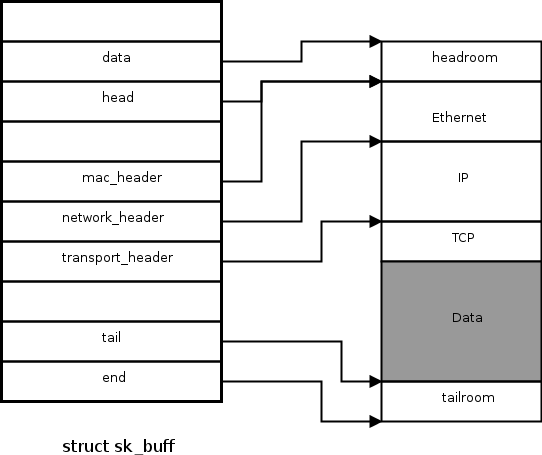
\includegraphics[width=9cm,keepaspectratio]{fig/skb.png}
	\caption{Socket buffer structure}
	\label{fig:linux-skb}
	\bigskip
\end{figure}

According to the {\it{protocol}} member, a pointer to the {\it{skb}}
of the received packet is passed to a higher-layer protocol handler.
In case of an IPv4 packet, it is the {\it{ip\_rcv()}} function,
which is part of the Linux IPv4 stack.
